\documentclass[11pt]{article}
\usepackage{amssymb}
\usepackage{amsthm}
\usepackage{amsmath}
\usepackage{listings}
\usepackage{color}
\usepackage{graphicx}
\usepackage{subcaption}
\usepackage[margin=1.0in]{geometry}

\lstdefinestyle{matlab-style}{
language=Matlab,
basicstyle=\scriptsize\ttfamily,
tabsize=2,
rulecolor=,
language=matlab,
basicstyle=\scriptsize,
aboveskip={1.5\baselineskip},
columns=fullflexible,
showstringspaces=false,
extendedchars=true,
breaklines=true,
prebreak = \raisebox{0ex}[0ex][0ex]{\ensuremath{\hookleftarrow}},
frame=single,
showtabs=false,
showspaces=false,
showstringspaces=false,
identifierstyle=\ttfamily,
keywordstyle=\color[rgb]{0,0,1},
commentstyle=\color[rgb]{0.133,0.545,0.133},
stringstyle=\color[rgb]{0.627,0.126,0.941},
keepspaces=true,
numbers=left,
numbersep=5pt,
numberstyle=\tiny\color[rgb]{0.5,0.5,0.5},
stepnumber=1
}

\newcommand{\bs}[1] {\boldsymbol{#1}}

\title{Design of an optimal wing spar\\MANE 6963 - Project 2}
\author{ID: 2168}
\date{}

\begin{document}

\maketitle
\tableofcontents
\newpage

\section{Executive summary}

\begin{figure}[hbt]
\centering
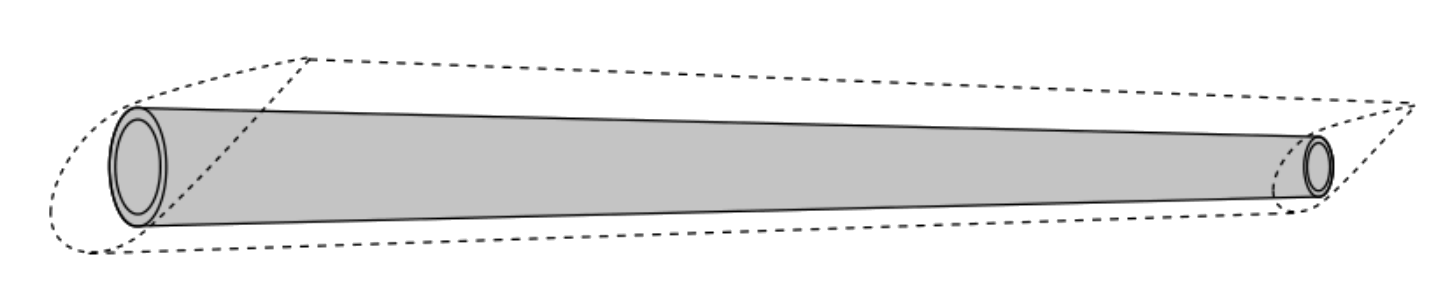
\includegraphics[width=0.6\textwidth]{spar}
\caption{Wing (dotted lines) and illustration of spar geometry}
\label{fig:spar}
\end{figure}

In this report, we investigate the optimal design of a
spar as the primary support for the wing of an aircraft.
Figure \ref{fig:spar} shows an illustration of the spar
that is to be designed. Our main objective is to minimize the
weight (and thus the mass) of the wing spar subject to
operational assumptions about the aircraft,
engineering design assumptions, and engineering
design constraints. These assumptions and
constraints are outlined below.

\subsection{Aircraft operational assumptions}

We assume that the total mass of the aircraft
is $m_{\text{plane}} = 500$ kg and that the weight
of the plane is equally supported by two wings.
Additionally, we assume that the plane is operating
at a $2.5$ g maneuver, where the span-wise force
distribution acting on the wing (and thus on the spar)
varies linearly, vanishing at the wing tip. The
distribution of this force per unit area $q(x)$
acting on the spar is shown in Figure \ref{fig:load}.

\begin{figure}[hbt]
\centering
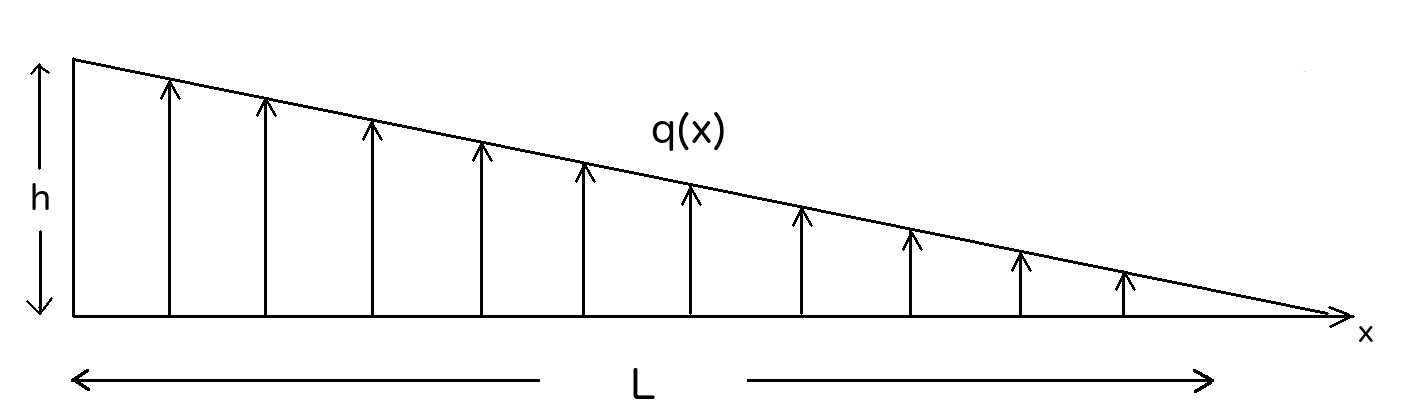
\includegraphics[width=0.6\textwidth]{load}
\caption{Load imposed on the wing}
\label{fig:load}
\end{figure}

\subsection{Engineering design assumptions}

We assume that the wing semi-span $L$ is $7.5$ m,
and that the spar supporting the wing will be made
of a carbon fiber composite material. The material properties
of the composite are listed in Figure \ref{fig:materials}.
Additionally, we assume that the cross-section of
the spar in the $yz$ plane is a circular annulus,
as shown in Figure \ref{fig:annulus}.

\begin{figure}[hbt]
\centering
\begin{tabular}{ | l | r  |}
\hline
Material property & Value \\ \hline
Density $(\rho)$ & $1600$ km/m$^3$ \\ \hline
Young's modulus $(E)$ & $70$ GPa \\ \hline
Ultimate yield strength $(Y)$ & $600$ MPa \\ \hline
\end{tabular}
\caption{Material properties of the spar}
\label{fig:materials}
\end{figure}

\subsection{Engineering design constraints}

Due to material manufacturing constraints, we
assume that the inner radius of the spar $r^i$ at all
points along the $x$-axis is greater than or equal to $1$ cm
and that the inner and outer radii of the spar cannot be
more than $2.5$mm apart.
Because the spar must remain within the wing, we
constrain the outer radius $r^o$ of the spar to be less
than or equal to $5$ cm.
Finally, we stipulate that the normal stress $\sigma$ at all
span-wise locations must be less than the yield
strength $Y$ in order to maintain a safe design.

\begin{figure}[hbt]
\centering
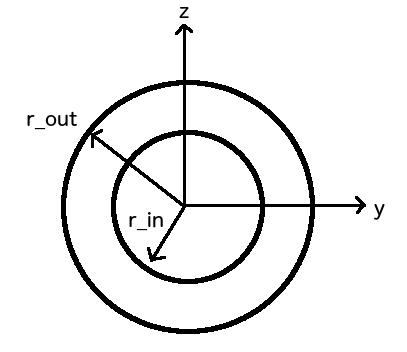
\includegraphics[width=0.3\textwidth]{annulus}
\caption{Annular cross-section of the spar geometry}
\label{fig:annulus}
\end{figure}

\subsection{Work done to achieve optimization goal}

To achieve the stated optimization goal subject to the above
constraints and assumptions, we have:
\begin{itemize}
\item Determined a suitable spar geometry parameterization,
defined by a design vector $\bs{p}$.
\item Derived the appropriate force per unit length function
$q(x)$ based on our design assumptions and implemented a Matlab
method CalcForce.m that evaluates $q(x)$ at discrete points.
\item Implemented a Matlab routine CalcMoment.m that computes
the second moment of area at cross-sections of the spar geometry.
\item Provided the functions CalcForce.m and CalcMoment.m to a
finite element analysis code to compute the normal stresses
$\sigma$ at discrete grid locations along the spar.
\item Implemented the Matlab routine CalcMass.m to compute
the mass $m$ of the spar as a function of the design variables
$\bs{p}$.
\item Implemented the Matlab routine Obj.m to compute the
mass objective function, as well as its gradient using
the complex-step method.
\item Implemented the Matlab routines ConstraintLower.m,
ConstraintUpper.m, and ConstraintStress.m to effectively
impose the necessary constraints.
\item Utilized Matlab's \emph{fmincon} routine, along with the methods
Obj.m, ConstraintLower.m, ConstraintUpper.m, and ConstraintStress.m,
to determine an optimal spar geometry.
\end{itemize}

In the remainder of this report, the mathematical and
implementation details of each item
in the list above are sequentially discussed.
Results of the optimization study are shown and finally
conclusions are drawn. The final optimal geometry shows a
$62$ percent reduction in mass over a chosen nominal
geometry. All Matlab routines named are listed
in the Appendix.

\section{Geometry parameterization}

As stated previously, each cross-section in the $yz$ plane of the
spar geometry is assumed to be a circular annulus. We discretize
the $x$-axis using $N_x$ grid points and assume that the spar
varies piecewise linearly along the $x$-direction from grid
point to grid point. An illustration of this piecewise linearly
varying geometry is shown in Figure \ref{fig:representation}.
We parameterize this geometry by a vector $\bs{p}$
that is the concatenated values of the
inner radii values $r^i_j$ and the annular thickness
$t_j = r^0_j - r^i_j$ evaluated at discrete grid points $x_j$,
where $j=1,2,\dots,N_x$. Thus, $\bs{p} \in \mathbb{R}^{2 N_x}$
has the layout
\begin{equation}
\bs{p} = [r^i_1, r^i_2, \dots r^i_{N_x}, t_1, t_2, \dots, t_{N_x}]^T
\end{equation}

\begin{figure}[hbt]
\centering
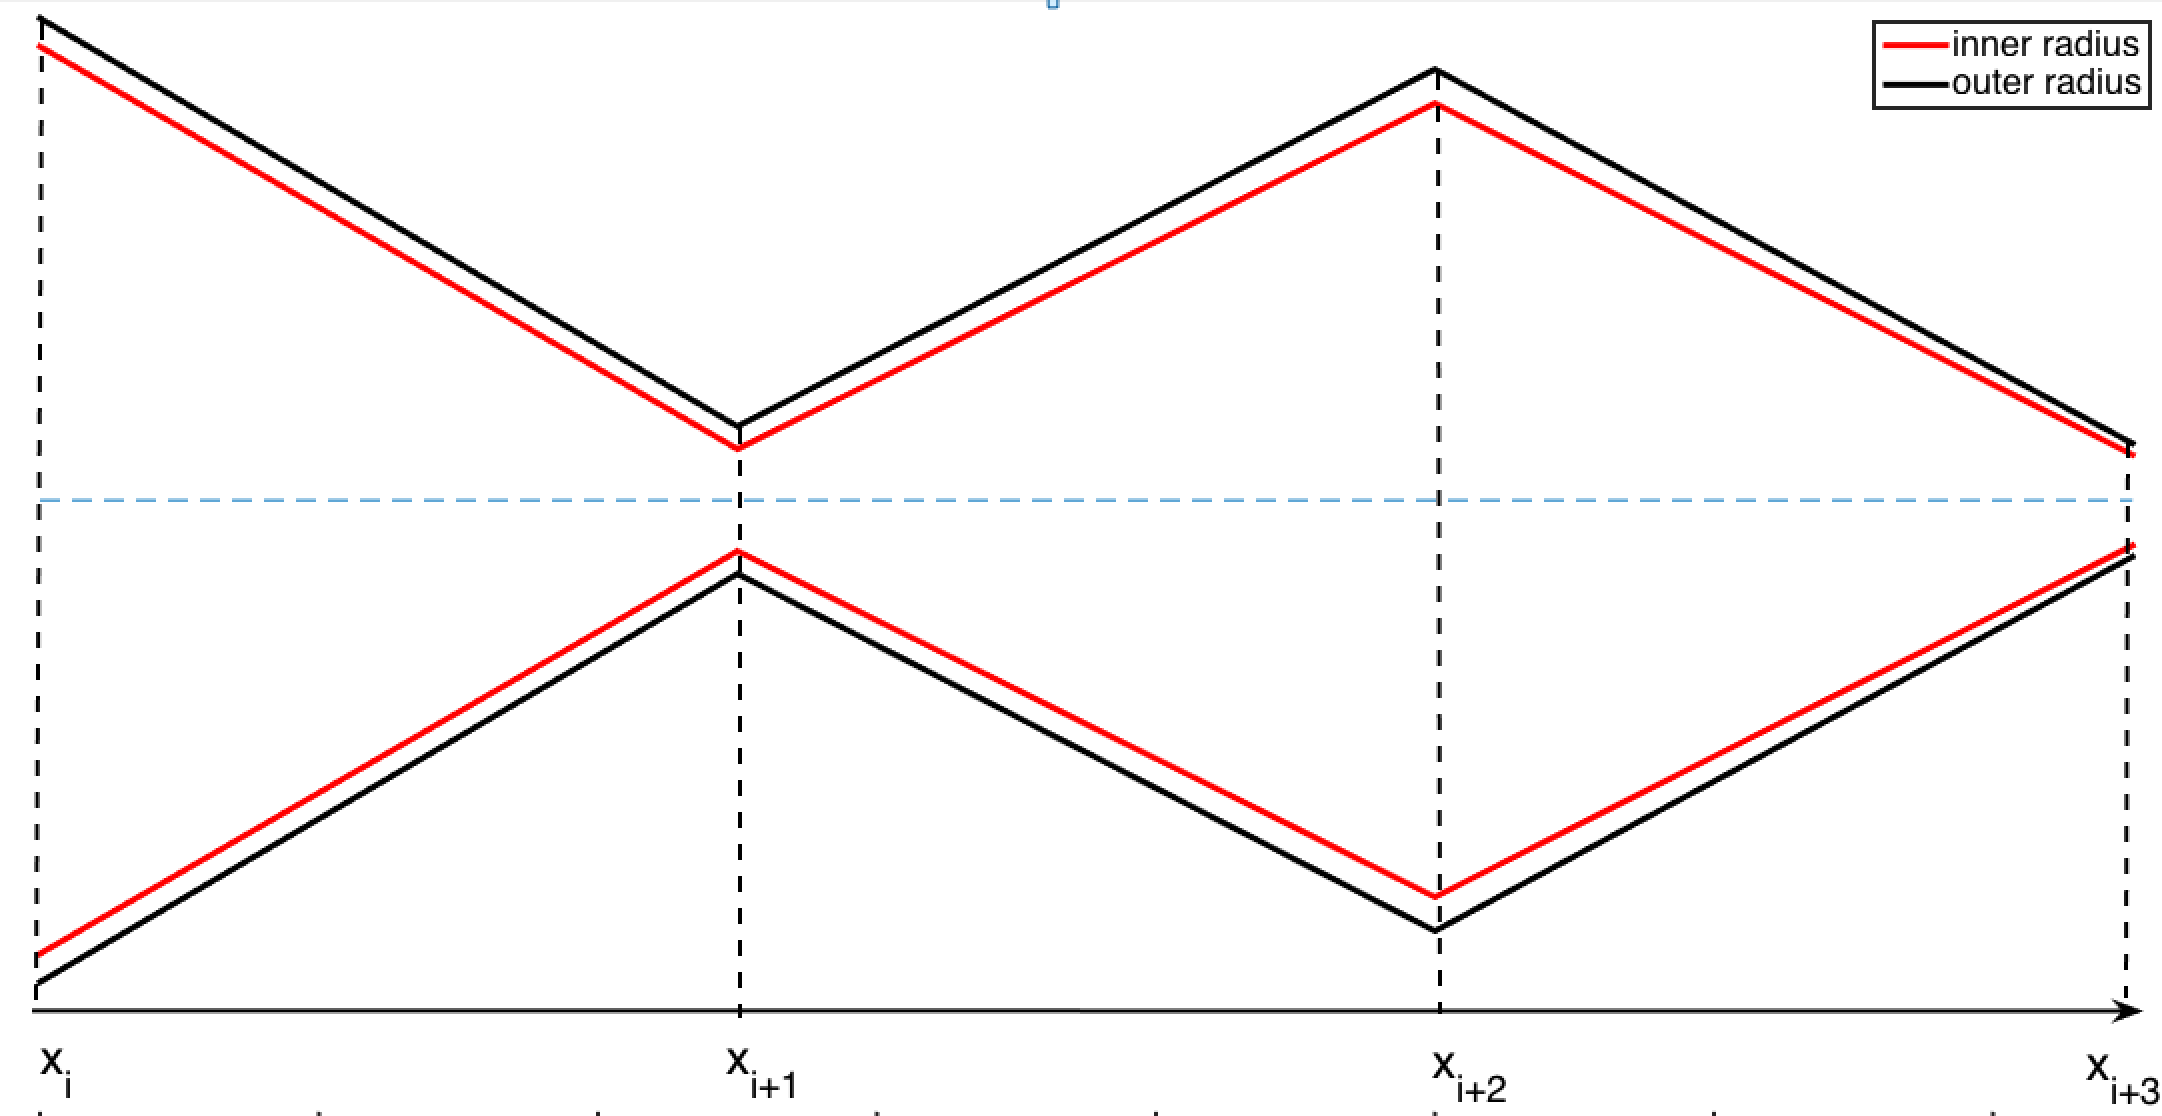
\includegraphics[width=0.5\textwidth]{representation}
\caption{Piecewise linear geometry representation}
\label{fig:representation}
\end{figure}

\section{Analysis methods}

\subsection{PDE Model}

We model the deformation of the wing spar using Euler-Bernoulli
beam theory, represented by the PDE:
\begin{equation}
\frac{d^2}{d x^2}
\left( E I_{yy} \frac{d^2 u}{dx^2} \right) =
q, \quad \forall x \in [0,L],
\label{eq:pde}
\end{equation}
where $I_{yy}$ is the second moment of inertia of the
cross-section of the spar and $q$ is an applied load.
We impose zero vertical displacement and zero angular
displacement boundary conditions where the spar connects
to the fuselage:
\begin{equation}
\begin{aligned}
u(x=0) &= 0, \\
\frac{du}{dx} (x=0) &= 0,
\end{aligned}
\end{equation}
and traction free boundary conditions at the spar tip:
\begin{equation}
\begin{aligned}
\frac{d^2 u}{dx^2} (x=L) &= 0, \\
\frac{d^3 u}{dx^3} (x=L) &= 0.
\end{aligned}
\end{equation}
Here, we have assumed that the material is elastic
and isotropic, i.e. $E$ does not vary spatially.
Additionally, we have assumed that the internal
strain accounts only for deformations due to
bending moments, and that these deformations are
small enough to neglect nonlinear effects.
Before presenting an appropriate numerical method to
solve this PDE, we first derive analytical expressions
for the load $q(x)$ and for the second moment of inertia
$I_{yy}$.

\subsection{Applied load}

It is known that the total force acting on a single wing,
and thus on a single spar, of the aircraft during the $2.5$
g maneuver is
\begin{equation}
F = (2.5)(9.8 \text{m}\text{s}^{-2})(\frac12)(500 \text{kg}) = 6125 \text{N}.
\end{equation}
It is also known that the total force $F$ applied to the
spar is given as
\begin{equation}
F = \int_0 ^L q(x) dx,
\end{equation}
the area under the curve in Figure \ref{fig:load} which
forms a triangular region. From geometry, we have $F = \frac12 h L$,
where $h$ is the height of the triangle. This implies that
$h = \frac{2F}{L}$.
Using the formula for a straight line, we conclude that
the expression for the force-per unit area is
\begin{equation}
q(x) = \frac{2F}{L} \left( 1 - \frac{x}{L} \right).
\end{equation}
The Matlab function CalcForce.m returns the value
of the force per-unit area $q(x)$ at discrete $x$
locations.

\subsection{Second moment of inertia}

As mentioned previously, the cross-section of the spar
geometry in the $xz$ plane is a circular annulus
(see Figure \ref{fig:annulus}). The second moment
of inertia for an annulus is given by the equation:
\begin{equation}
I_{yy} = \iint z^2 \text{d} z \text{d} y.
\end{equation}
Basic calculus leads to the result:
\begin{equation}
I_{yy} = \frac{\pi}{4} \left ( (r^o)^4 - (r^i)^4 \right).
\end{equation}
The Matlab function CalcMoment.m returns the value
of $I_{yy}$ at discrete $x$-locations along the spar.

\subsection{Finite element analysis}

The model PDE \eqref{eq:pde} is solved with a finite
element method using Hermite cubic shape functions.
The domain is consistently discretized with the geometry
representation, where $N_x-1$ elements are used. The interval
$[0,L]$ is split into the discrete points
$\{ x_1, x_2, \dots, x_{N_x} \}$, where the $j^{th}$
element is defined over the interval $x_{j+1} - x_j$.
We assume that the element length $\Delta x = x_{j+1} - x_j$
is uniform for all elements, $j=1,2,\dots,N_x-1$.
The previously described methods CalcForce.m and
CalcMoment.m are utilized by the finite element analysis
to determine the values of $q(x)$ and $I_{yy}$, respectively,
at discrete $x_j$ locations. The finite element analysis
computes the displacements $u_j$ at discrete grid locations.
These displacements are then post-processed to determine
the stresses $\sigma_j$ at discrete points.

\section{Optimization methods}

\subsection{Computation of spar mass}

Our main objective is to minimize the weight, and thus
the mass $m$ of the spar. To compute the mass of the
spar, we first compute the spar's volume. The total volume
of the spar is computed as the sum of the volume computed
over each element in the discrete domain:
\begin{equation}
V = \sum^{N_x-1}_{j=1} V^o_j - V^i_j
\end{equation}
where $V^o_j$ denotes the volume of the truncated cone
defined by the values of the spar's outer
radii values at $x_j$ and $x_{j+1}$
\begin{equation}
V^o_j = \frac{\pi \Delta x}{3} ((r^o_j)^2 + (r^o_{j+1})^2 + (r^o_j)(r^o_{j+1})),
\end{equation}
and $V^i_j$ denotes the volume of the truncated cone
defined by the values of the spar's inner
radii values at $x_j$ and $x_{j+1}$
\begin{equation}
V^i_j = \frac{\pi \Delta x}{3} ((r^i_j)^2 + (r^i_{j+1})^2 + (r^i_j) (r^i_{j+1})).
\end{equation}
Naturally, the difference $V^o_j-V^i_j$ denotes the
total volume associated with the element defined
by the points $x_j$ and $x_{j+1}$.
The mass of the spar is then simply computed
as the material density $\rho$ times the spar's volume:
\begin{equation}
m(\bs{p}) =  \rho V(\bs{p}),
\end{equation}
where we have noted the dependence of the mass on the parameter
vector $\bs{p}$. The Matlab
function CalcMass.m returns the computed value
of the spar's mass, given inner and outer radii
values at discrete grid locations.

\subsection{Optimization problem statement}

Using the previous definition of the spar's mass $m$ and the
definition of the parameter vector $\bs{p}$, the
optimization problem of interest can be stated:
\begin{equation}
\begin{aligned}
& \underset{\bs{p}}{\text{minimize}}
& & m(\bs{p}) \\
& \text{subject to}
& & p_j \geq 0.01,                    &j=1,2,\dots,N_x \\
&&& p_{N_x+j} \geq 0.0025,            &j=1,2,\dots,N_x\\
&&& p_j + p_{N_x +j} \leq 0.05,       &j=1,2,\dots,N_x \\
&&& \sigma_j(\bs{p})/Y \leq 1.0,      &j=1,2,\dots,N_x
\end{aligned}
\end{equation}
Here, we note that the first constraint is the lower bound
constraint on the inner radius, $r^i \geq 1$ cm. Similarly,
the second constraint corresponds to the thickness lower
bound constraint $t \geq 2.5$ mm. These two lower bound
constraints are implemented in the Matlab routine
ConstraintLower.m. The third constraint states that the
outer radius $r^o$ must not exceed $5$ cm, and is implemented
as a linear inequality constraint in the Matlab function
ConstraintUpper.m.

The final constraint prohibits the
stress $\sigma$ at all points in the domain from exceeding
the yield strength $Y$ and is implemented as a nonlinear
constraint in ConstraintStress.m. Note that we have scaled
this nonlinear constraint by dividing both sides by the
yield strength $Y$ so that all constraints are closer
to the same order of magnitude.
Additionally, we compute the nonlinear
constraint Jacobian on line 31 of ConstraintStress.m
using the complex step method, where
\begin{equation}
[ \nabla c ]_{kj} = \frac{\partial \sigma_j / Y}{\partial p_k}
\end{equation}
Finally, note that
nonlinear constraint is dependent on the stress results
$\sigma_j$ obtained from the finite element analysis.

\subsection{Optimization methods}

The optimization problem statement is fully encapsulated
in the Matlab script Driver.m. We utilize $N_x=40$ grid
points in the finite element analysis to ensure accurate
results. As a result, there are $N_p=80$ total design
variables. The Matlab routine Obj.m is a wrapper around
the method CalcMass.m, that returns the value of the
mass objective function $m(\bs{p})$ as well as its
gradient $\nabla m(\bs{p})$, which is computed using
the complex step method. The complex-step method
computation begins on line $23$ of Obj.m, and computes the
components of the gradient in the following manner:
\begin{equation}
[ \nabla m(\bs{p}) ]_j = \frac{\text{Im}(m( \bs{p} + i h \bs{e}_j))}{h},
\quad j=1,2,\dots,N_p,
\end{equation}
where $h$ is the chosen-step size for the method. Note
on line $31$ of Driver.m, we choose this step-size
to be $h=1e-30$. 

We utilize gradient based optimization techniques through
Matlab's \emph{fmincon} routine. We choose a
sequentially quadratic programming algorithm.
We choose Matlab's default convergence tolerances
for \emph{fmincon} as they are suitably accurate
for our purposes.
Additionally, we ensure that we utilize the gradient
determined by the complex-step method and the
nonlinear constraint Jacobian determined by the
complex step method, rather than
\emph{fmincon}'s own finite differencing schemes.
This can be seen on lines $46$ and $47$ of Driver.m 

\section{Results}

The program Driver.m was run as it is currently presented
in the Appendix. We choose the initial guess $\bs{p}_0$ to
optimization algorithm such that $r^o = 5$ cm and $r^i = 4.635$ cm
at all grid points. We refer to the geometry configuration defined
by this initial guess as the \emph{nominal} geometry.
The convergence history for the optimization
problem is shown in Figure \ref{fig:convergence}.

\begin{figure}[hbt!]
\small
\centering
\begin{verbatim}
                                                          Norm of First-order
 Iter F-count            f(x) Feasibility  Steplength        step  optimality
    0       1    1.325793e+01   0.000e+00                           9.666e+01
    1      10    1.301465e+01   0.000e+00   8.235e-02   1.460e-02   9.666e+01
    2      12    5.936808e+00   9.481e-01   7.000e-01   1.291e-01   6.879e+01
    3      13    4.744577e+00   9.421e-01   1.000e+00   4.625e-02   5.294e+01
    4      14    4.887080e+00   2.540e-01   1.000e+00   7.417e-03   1.233e+01
    5      15    4.911823e+00   3.159e-02   1.000e+00   1.995e-03   2.024e+00
    6      16    4.913419e+00   5.580e-04   1.000e+00   2.287e-04   1.517e-01
    7      17    4.913433e+00   1.534e-07   1.000e+00   4.053e-06   1.812e-03
    8      18    4.913433e+00   1.244e-11   1.000e+00   1.342e-09   2.160e-06
\end{verbatim}
\caption{Convergence results for geometry optimization}
\label{fig:convergence}
\end{figure}

Note that
the function call count \emph{F-count} is scaling directly
with the number of iterations. This gives us confidence that
\emph{fmincon} is utilizing the supplied objective gradient and
the nonlinear constraint Jacobian.

\begin{figure}[hbt!]
\centering
\begin{minipage}[b]{0.4\textwidth}
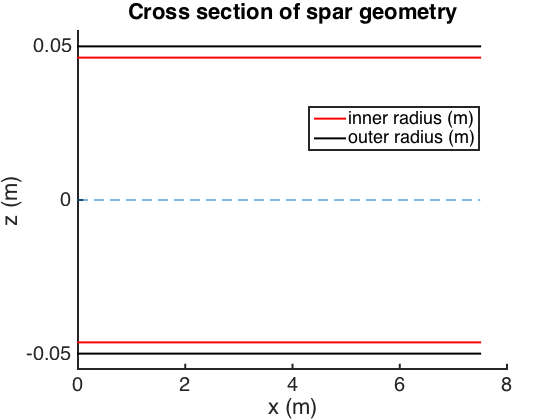
\includegraphics[width=0.9\textwidth]{nominal_geom}
\caption{Nominal spar geometry}
\label{fig:nominal_geom}
\end{minipage}
\begin{minipage}[b]{0.4\textwidth}
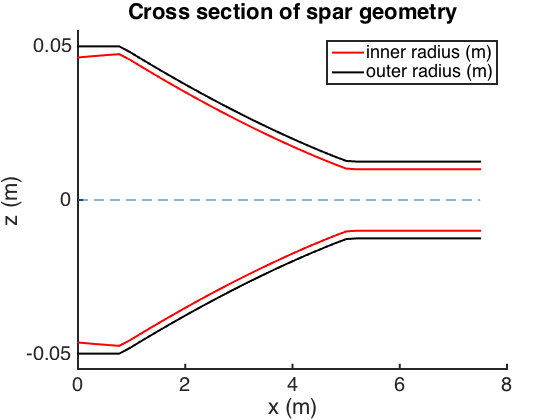
\includegraphics[width=0.9\textwidth]{optimal_geom}
\caption{Optimal spar geometry}
\label{fig:optimal_geom}
\end{minipage}
\end{figure}

The cross-section of the geometry in the $xz$-plane
for the nominal geometry and for the optimal
geometry are shown in Figures \ref{fig:nominal_geom}
and \ref{fig:optimal_geom}, respectively.
We note that the thickness of the spar is smaller for
the optimal geometry than for the nominal geometry
at nearly all span-wise locations. This is congruent
with the design intuition that the optimal geometry
should use the least amount of material, while still
satisfying the minimum thickness constraint. Additionally,
the inner and outer radii constraints, $r^i \geq 1$ cm
and $r^o \leq 5$ cm, respectively, are clearly
satisfied, further increasing our confidence that
the optimal geometry has been found.

\begin{figure}[hbt!]
\centering
\begin{minipage}[b]{0.4\textwidth}
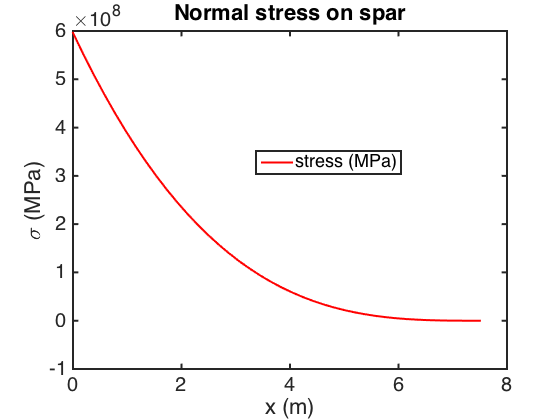
\includegraphics[width=0.9\textwidth]{nominal_stress}
\caption{Nominal stress distribution}
\label{fig:nominal_stress}
\end{minipage}
\begin{minipage}[b]{0.4\textwidth}
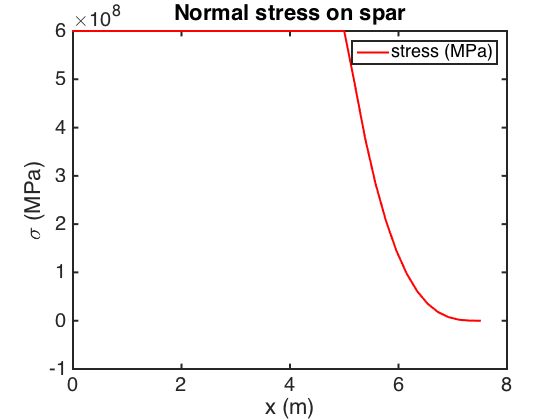
\includegraphics[width=0.9\textwidth]{optimal_stress}
\caption{Optimal stress distribution}
\label{fig:optimal_stress}
\end{minipage}
\end{figure}

Similarly, the stress distributions obtained when the
load $q(x)$ is applied to the nominal geometry and to
the optimal geometry are shown in Figures
\ref{fig:nominal_stress} and \ref{fig:optimal_stress},
respectively. Again, the results for the stress
distribution align with the engineering intuition
that the material should be pushed to its yield
strength $Y = 600$ MPa, but no further. The stress
distribution along the $x$-axis begins to decrease
at around $5$ m because, at this point, the
inner radii constraint has been met, and can get
no smaller.

Finally, we note that the computed mass of the
optimal spar geometry is found to be
$4.91$ kg. This is about a  $62$ percent
reduction over the nominal mass value of $13.26$ kg.

\section{Conclusions}

In conclusion, we have used constrained gradient based
optimization to determine the geometry of a
wing spar. The spar is optimal in the sense that its
geometry minimizes the mass of the spar, and thus
its weight, subject to various engineering assumptions
and constraints. We have made use of the accurate
complex-step method within our optimization algorithm.
The optimal geometry saw a $62$ percent reduction
in mass when compared to a nominal geometry.

\newpage

\section{Appendix: code listings}

\lstinputlisting[style=matlab-style,caption=CalcForce.m]{CalcForce.m}
\lstinputlisting[style=matlab-style,caption=CalcMoment.m]{CalcMoment.m}
\newpage
\lstinputlisting[style=matlab-style,caption=CalcMass.m]{CalcMass.m}
\lstinputlisting[style=matlab-style,caption=ConstraintLower.m]{ConstraintLower.m}
\newpage
\lstinputlisting[style=matlab-style,caption=ConstraintUpper.m]{ConstraintUpper.m}
\lstinputlisting[style=matlab-style,caption=ConstraintStress.m]{ConstraintStress.m}
\newpage
\lstinputlisting[style=matlab-style,caption=Obj.m]{Obj.m}
\newpage
\lstinputlisting[style=matlab-style,caption=Driver.m]{Driver.m}

\end{document}
